\chapter{Dettagli tecnici}

\section{Rete Neurale}

Una Rete Neurale è un modello matematico che simula il funzionamento della mente biologica umana, ed è utilizzata per tentare di risolvere problemi ingegneristici di intelligenza artificiale. \cite{wiki_nn}

Nel nostro caso, per la risoluzione di problemi di visione artificiale, utilizzeremo le reti neurali multi livello (o multi layer), chiamate anche MLP (Multi Layer Perceptron), che appartengono ad una sotto categoria del Machine Learning chiamata Deep Learning.

Da notare che non tutti i modelli di Intelligenza Artificiale sono basati sulle reti neurali; esistono anche altre tecnologie utilizzate nel mondo del Machine Learning come i Decision Trees,
i quali creano diagrammi di flusso basati su condizioni specifiche, oppure le Random Forest, cioè l'unione di più Decision Tree indipendenti. \\

\begin{figure}[htbp]
    \centering
    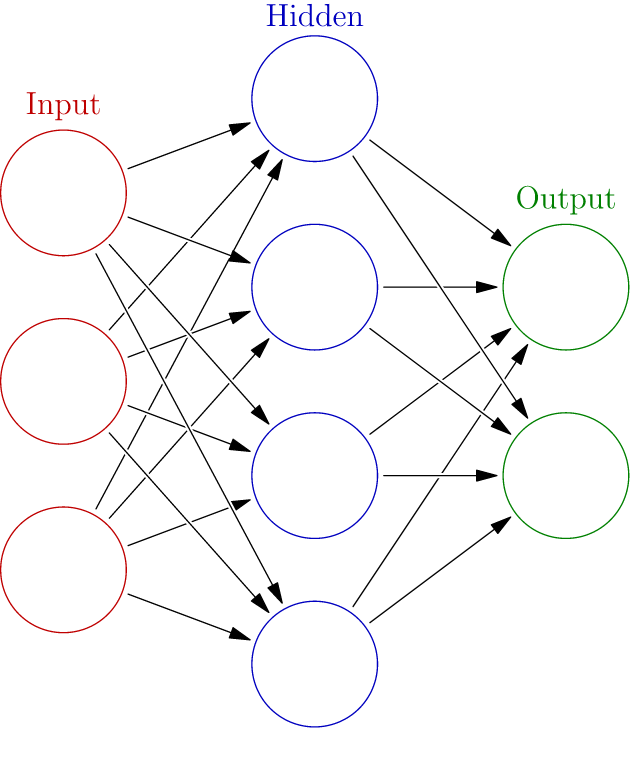
\includegraphics[width=0.45\textwidth]{images/neural_network.png}
    \cite{wiki_nn_image}
    \caption{Percettrone Multistrato}
    \label{fig:neural_network}
\end{figure}

\newpage

\subsection{Layers}

In una Rete Neurale i layers rappresentano i diversi strati della rete. In ogni strato sono presenti uno o più neuroni chiamati unità. \\

\noindent
Sono generalmente presenti tre strati :
\begin{enumerate}
    \item Input : con unità che rappresentano i campi di input.
    \item Hidden Layers : con uno o più strati.
    \item Output : con una o più unità che rappresentano i campi obiettivo.
\end{enumerate}

\noindent
I dati di input vengono presentati nel primo strato e i valori vengono propagati da ciascun neurone a ogni neurone nello strato successivo, ed alla fine viene fornito un risultato nello strato di output. \cite{ibm_neural_model}

\subsection{Pesi}

Le unità sono connesse con varie intensità di connessione, dette \hypertarget{weights}{pesi}.

Tutti i pesi inizialmente sono casuali e le risposte ottenute dalla rete risulteranno probabilmente prive di senso.

La rete apprende generando una previsione per ogni input dato e correggendo i pesi ogni volta che viene sbagliata una previsione.
Questo processo, anche detto \hyperlink{epoch}{\textit{epoca}}, viene ripetuto molte volte e la rete continua a migliorare le sue previsioni finché uno o più criteri di interruzione non vengono soddisfatti. \cite{ibm_neural_model}

\subsection{Bias}

Il parametro di \hypertarget{b}{bias} è quello che, durante il calcolo matematico che avviene all'interno della singola unità (neurone) permette di aggiungere un'errore al modello,
considerato troppo semplice, con l'obbiettivo di catturare una maggiore complessità dei dati.

\newpage

\section{Dataset}
Un Dataset è una raccolta strutturata di dati, che in questo caso servirà per la fase di addestramento (training) dei nostri modelli. \\

\noindent
In generale, un Dataset per l'addestramento di Reti Neurali è suddiviso in :
\begin{itemize}
    \item Training set : immagini usate per il training del nostro modello.
    \item Validation set : immagini utilizzate durante l'addestramento, per valutare le prestazioni del modello su dati non visti e per effettuare la messa a punto dei parametri.
    \item Test set : un insieme di immagini utilizzate alla fine dell'addestramento, per valutare le prestazioni finali del modello, su dati completamente nuovi che non sono stati utilizzati per il training.
\end{itemize}

Il Validation set è opzionale, ma molto utile per migliorare la qualità del training del modello.

\subsection{Qualità di un Dataset}
La qualità di un Dataset è data dalla correttezza delle sue annotazioni, cioè dalla coerenza di quello che mi stanno dicendo i dati al suo interno, ma anche dalla varietà dei dati al suo interno,
perché avrò molti più esempi da mostrare al mio modello nella fase di addestramento.

Perciò se i dati sono coerenti ai problemi del mondo reale di cui si occuperà il modello, impararne i pattern e le correlazioni consentirà al modello addestrato di fare previsioni accurate su nuovi dati.

\newpage

\section{Training}

L'addestramento di un modello è la fase del Machine Learning (ML) in cui avviene l'apprendimento. Nel ML, l'apprendimento implica la regolazione dei parametri di un modello ML.
Questi parametri includono \hyperlink{weights}{\textit{pesi}} e \hyperlink{b}{\textit{bias}} nelle funzioni matematiche che costituiscono i loro algoritmi.

Durante questa fase, ogni volta che un input arriva ad un nodo, viene moltiplicato per il peso (weight) associato a quella specifica connessione,
e la somma di tutti questi input con un certo valore di bias ne determinerà poi i valori in output.

Dal punto di vista matematico, l'obiettivo di questo apprendimento è quello di ridurre al minimo una funzione di perdita che quantifica l'errore degli output nelle attività di addestramento.
Quando l'output della funzione di perdita scende al di sotto di una soglia predeterminata, ovvero l'errore del modello nelle attività di addestramento è sufficientemente piccolo,
il modello viene considerato "addestrato". \cite{training_nn}

\subsection{Training from scratch}

In questa tipologia di training, il modello viene addestrato su dati annotati senza partire da pesi pre-trainati, quindi senza usare come base un modello già allenato.

Partendo da zero, ovvero from scratch, i pesi non sono definiti ma vengono assegnati dei numeri casuali che, soltanto durante il processo di training, verranno modificati per ottimizzare le prestazioni.

Questo tipo di training è valido quando abbiamo a disposizione un numero considerevole di dati annotati e l'utilizzo del modello è molto specifico.

\subsection{Transfer Learning}

In scenari caratterizzati da dataset limitati o per ottimizzare tempi e risorse computazionali, è prassi comune ricorrere al transfer learning, inizializzando la rete con pesi pre-addestrati.

Questo approccio si fonda sulla natura gerarchica dell'apprendimento profondo: i primi layer della rete estraggono caratteristiche universali delle immagini, come bordi, variazioni di colore, e texture,
mentre solo gli strati più profondi si specializzano su task specifici.
Sfruttando la rappresentazione generale appresa precedentemente su dataset massivi, si evita di dover ricostruire l'estrattore di feature da zero, concentrando il nuovo addestramento solo su ciò che è strettamente legato al nuovo dominio.

I vantaggi rispetto a un addestramento from scratch sono notevoli: una drastica riduzione dei dati annotati necessari, una convergenza più rapida, con conseguente abbattimento dei costi computazionali,
ed infine migliore capacità di generalizzazione.
Il limite principale è invece legato al cambio di dominio, dove il trasferimento di conoscenza perde di efficacia se il nuovo dominio si discosta eccessivamente da quello di partenza.

\subsection{Fine-tuning}
\label{sec:fine_tuning}

Mentre il transfer learning rappresenta il paradigma concettuale, il fine-tuning ne costituisce l'implementazione pratica, in cui l'addestramento non parte da pesi inizializzati casualmente,
ma da uno stato pre-ottimizzato che viene gradualmente adattato al nuovo dominio di riferimento.
Operativamente, si distinguono due approcci: nel fine-tuning \textit{completo} l'intera architettura viene aggiornata, garantendo massima flessibilità a fronte di un elevato onere computazionale;
nel fine-tuning \textit{parziale}, invece, i layer iniziali vengono "congelati" per preservare l'estrazione di feature generali, limitando l'aggiornamento agli strati terminali, spesso sostituiti per adattarsi alle nuove classi.

Un aspetto critico in questo processo è la calibrazione del learning rate, che deve essere sensibilmente inferiore rispetto al training from scratch.
Aggiornamenti troppo aggressivi distruggerebbero infatti i delicati equilibri dei pesi originali, innescando il cosiddetto \textit{catastrophic forgetting}, cioè la perdita irreversibile della conoscenza pregressa.
Al contempo, occorre bilanciare attentamente la durata dell'addestramento per non incappare nell'overfitting, specialmente se il nuovo dataset è di dimensioni ridotte.

Infine, l'enorme scala raggiunta dai recenti modelli linguistici e multimodali ha reso spesso quasi impraticabili gli approcci tradizionali.
Sono così emerse le tecniche di Parameter-Efficient Fine-Tuning (PEFT), che ottimizzano solo una frazione infinitesimale dei pesi mantenendo inalterata l'architettura originale.
Una delle metodologie più efficaci in questo ambito è LoRA, approfondita nella Sezione~\ref{sec:lora}.

\newpage

\section{Epoca}
Un'\hypertarget{epoch}{epoca} rappresenta un passaggio completo del dataset attraverso l'algoritmo in fase di learning, è un concetto fondamentale nel training delle reti neurali,
che permette al modello di imparare continuando costantemente a rivedere le stesse immagini, o i medesimi elementi del dataset.

Il numero di epoch si specifica solitamente in ogni procedura di training e determina quante volte il modello imparerà dal set di train del dataset, influenzando le performance e la qualità del modello.\\

\noindent
Scegliere il numero di epoch corretto è molto importante perché se viene scelto in maniera errata può creare due problemi:
\begin{itemize}
    \item Underfitting: il modello non è stato trainato per un numero sufficiente di epochs.
    Le performances non sono adeguate né sul set di training né su quello di test.
    
    \item Overfitting: il modello è stato trainato per troppi epochs.
    In questo caso memorizza i dati di training in maniera troppo approfondita e perde le sue abilità di analizzare i nuovi dati. Ha una precisione eccellente sul training set ma scarsa sul dataset di validazione.
\end{itemize}

Una tecnica comune per evitare l'overfitting è quella dell'early stopping, nella quale il training viene fermato quando le performances sul set di validazione smettono di migliorare.
A volte è possibile specificare un parametro chiamato patience, che specifica dopo quanti epochs "non migliorativi" il training deve fermarsi. \cite{epoch_ultralytics}.
